%% Copyright 1998 Pepe Kubon
%%
%% `one.tex' --- 1st chapter for thes-full.tex, thes-short-tex from
%%                the `csthesis' bundle
%%
%% You are allowed to distribute this file together with all files
%% mentioned in READ.ME.
%%
%% You are not allowed to modify its contents.
%%

%%%%%%%%%%%%%%%%%%%%%%%%%%%%%%%%%%%%%%%%%%%%%%%%%
%
%       Chapter 3
%
%%%%%%%%%%%%%%%%%%%%%%%%%%%%%%%%%%%%%%%%%%%%%%%%

\chapter [Propositionalization for Outlier Detection]{Propositionalization for Unsupervised Outlier Detection in Object-relational Data}\label{chap:four}

	In this chapter we develop a novel propositionalization  approach to unsupervised outlier detection for object-relational data. Propositionalization summarizes the information from relational data, that is typically stored in multiple tables, into a single data table. An advantage of propositionalization is that it facilitates leveraging the many previous outlier detection methods that were designed for single-table data. 
	Previous work has employed propositionalization for various applications; Anderson {\em et. al} ~\cite{Anderson2007} use propositionalization to apply clustering algorithms, like KMeans, to multi-relational data. Propositionalization for classification has been extensively explored~\cite{Kramer2000,Lavrac13,Lavravc2014,kuzelka2008}. ODDBALL extracts patterns from large weighted graphs and then uses those patterns as features to discover anomalous nodes in graph~\cite{Akoglu2010}.
	
	In this work we develop propositionalization for outlier detection for the case of object-relational data. 
	A novel application of Markov Logic Network structure learning is the basis of our propositionalization method for outlier detection. 
	%
	Alternative propositionalization methods that we evaluate in this work are based on enumerating all conjunctive formulas with, at most, two literals (unigrams and bigrams). 
	Compared to baseline propositionalization methods, Markov Logic propositionalization produces the most compact data tables whose attributes capture the most complex object-relational correlations. (More complex correlations are represented by longer logical formulas). We apply three representative outlier detection methods ($\lof$, $\knn$, $\outrank$) to the data tables constructed by %Markov Logic 
	propositionalization.
	%	The data tables produced by Markov Logic propositionalization capture the most complex multi-relational correlations, and were substantially more compact (half the dimensionality or less) which led to substantially faster runtimes for the outlier detection methods (twice as fast or more). 
	For each outlier detection method, Markov Logic propositionalization provided the best average accuracy over all datasets compared to the baseline propositionalization methods.
		\section{Introduction} Many outlier detection methods have been developed for data that is represented in an attribute-value format \cite{aggarwal2013}. 
		This work addresses outlier detection for object-relational data. In a single data table a row represents a data point, a column represents an attribute of a data point, and a table entry represents an attribute value for a data point. 
		%In contrast, multi-relational data are ususally represented in multiple interrelated tables. 
		Data analysis tools that are built for single data tables, can be leveraged for multiple relational data tables via a pipeline approach: first, convert the object-relational data to a single attribute-value table, then apply the data analysis tool. Since the attribute value representation corresponds to propositional logic, the conversion process is called {\em propositionalization} \cite{Kramer2000}. 
		%This paper presents a novel propositionalization method for outlier detection with multi-relational data. 
		While propositionalization for classification has been extensively explored~\cite{Kramer2000,Lavrac13,Lavravc2014,kuzelka2008}, to our knowledge propositionalization for outlier detection is a new research problem.
		
		\paragraph{Approach.} We use Markov Logic Network (MLN) structure learning to construct a single data table from object-relational data. This is a novel application of MLN learning. The format of the resulting data table is an individual-centric representation~\cite{Lippi2011,Lavrac13}:  we assume that there is a target class of individuals to be ranked as potential outliers (e.g. soccer players or movies). A row in the data table represents the attributes of an individual. Attributes are defined by logical first-order formulas~\cite{Lippi2011}. The more complex the formula, the more relational information is represented by the formula. 
		A feature function maps an individual and a first-order formula to a real value that is the value of the attribute for the individual. For example, we use the number of instantiations or groundings of a formula as such a function. 
		%
		A Markov Logic Network structure is a set of formulas.  Our Markov Logic propositionalization method applies the MLN structure learning method, introduced in chapter~\ref{chap:three}, to produce a set of formulas, these formulas define attributes for propositionalization. Our approach can be summarized by this equation:\\
		
	%	\begin{displaymath}\label{eq:formulaEssen}
			  {  \em Markov Logic Network Structure = Set of Formulas = Set of Attributes }  (4.1)\\
%		\end{displaymath}


		A baseline comparison method is to enumerate all conjunctive formulas up to a fixed length $n$ as attributes for propositionalization.  This is an instance of the recent Wordification approach to propositionalization \cite{Lavrac13}. 
		Wordification is based on an analogy between text data and relational data, where an $n$-gram in text data corresponds to a conjunctive formula with $n$ literals. In text analysis, $n$-grams are often treated as features of a document. 
		Analogously, wordification uses conjunctive formulas up to a fixed length $n$ as features for propositionalization. 
		The disadvantage of this approach is that the number of such formulas grows exponentially with $n$. 
		
		\paragraph{Evaluation.}% Our code and datasets are available on-line at \cite{url}. 
		%
		We use synthetic and real-world datasets that were introduced in chapter~\ref{chap:three}. Markov Logic propositionalization produces significantly fewer attributes, leading to much smaller  data tables for outlier analysis compared to the baseline wordification approach. The MLN attributes capture more complex relational associations 
		% (half the number of columns or less). 
		(with over 3 literals on average compared to 2 literals for wordification). 
		%Using the $\auc$ accuracy metric,
		%, which is standard for outlier detection, 
		MLN propositionalization is competitive with wordification: for a given outlier analysis method,~%(one of $\lof$, $\knn$, $\outrank$), 
		the average $\auc$ score over all datasets is best for MLN propositionalization.
		
		We believe that propositionalization for outlier detection is a fruitful application area for other statistical-relational learning generative models in addition to Markov Logic Networks. 
		Our approach can  utilize %structure learning for 
		any model class whose structure is represented by logical formulas, or can be easily converted to logical formulas, which includes many statistical-relational models~\cite{Ravkic2015,Cussens2012,Kersting2007,SRL2007}.
		
		\paragraph{Contributions.} The contributions of this chapter may be summarized as follows. 
		
		\begin{enumerate}
			\item A novel task for relational learning: propositionalization for outlier detection. This facilitates leveraging standard single-table outlier analysis methods for object-relational data.
			\item A novel application of Markov Logic Network structure learning to perform this task. MLN structure learning generates a compact yet expressive set of features from object-relational data.
		\end{enumerate}
%			\section{Related Work} 
%			\paragraph{Propositionalization} 
%			has been explored extensively for classification tasks \cite{Kramer2000,Lavrac13,Lavravc2014,kuzelka2008}. We are not aware of previous work on propositionalization for {\em outlier detection.}  The wordification framework \cite{Lavrac13} introduces an analogy between the grounding counts of a formula and the frequency of a term in a document. Lavrac {\em et al.} apply this analogy for propositionalization for classifiers, which is implemented in the ClowdFlows system~\cite{Kranjc2012}. The $n$-gram methods in this chapter apply the analogy for outlier detection. 
%			
%			In previous applications of single-table outlier analysis methods to structured data, the data were manually propositionalized, by aggregating information about single attributes. 
%			For example, Breunig {\em et al.} counted the total number of goals scored by a player in a season as a attribute for outlier analysis by $\lof$\cite{Breunig2000}. Counts for single attributes in isolation are basically equivalent to the unigram-term frequency method that we evaluate in our experiments. Manual propositionalization is limited because it becomes very difficult for attributes that represent interactions between features (e.g., the bigram method below).
%			
%			
%			\paragraph{Relational Outlier Detection} has previously been based on discovering rules that represent the presence of anomalous associations for an individual or the absence of normal associations \cite{Novak2009,Maervoet2012}. 
%			%	Several deviation measures have been proposed for association rules \cite{Novak2009}.
%			Related work includes exception mining, which looks for associations that characterize unusual cases, subgroup mining, which looks for associations  characterizing important subgroups, and contrast space mining, which looks for differences between classes.  Novak {\em et al.}~\cite{Novak2009} show that these tasks can be unified as instantiations of a general rule search framework. None of the rule search methods use propositionalization. We were not able to obtain rule search implementation code for empirical comparison. 
%			
%			The community distribution approach \cite{Gupta2013} assumes a vector for each entity that indicates membership probabilities in different communities. Outliers can then be defined similar to the non-relational feature vector setting. Markov Logic propositionalization utilizes information from entities and links of different types, but does not assume that latent communities have been identified. 
%			
%						\paragraph{Inductive Logic Programming} has been used for relational outlier detection. One approach views an example as anomalous if it is not covered by a learned set of rules \cite{Angiulli2007}. Another measures the difference in generality between a rule set learned with the anomalous examples, and a rule set learned without ~\cite{Angiulli2009}. Neither performs propositionalization. No code is available for empirical comparison.
%%				
%				\section{Background and Notation} 
%				
%				We use notation and terminology from previous work \cite{Chiang2012,Lippi2011,Domingos2009}. While we do not introduce any new terminology, we combine concepts from different areas, such as propositionalization and log-linear models. We follow the description of propositionalization in Lippi {\em et al.} \cite{Lippi2011}, where the input to a propositionalizer is a relational database, and the output is a pseudo-\iid data view. 
%				
%%				\subsection{Predicate Language}
%%				
%%				We employ the notation of Chiang and Poole \cite{Chiang2012} for logical syntax, as follows.
%%				%
%%				Constants are expressed in lower-case, e.g. $\it{joe}$, and are used to represent individuals. A type is associated with each individual, e.g. $\it{joe}$ is a person. We use $D(\tau)$ to represent a domain of type $\tau$, which is the set of individuals of type $\tau$. A {\em logical variable} is written in upper case. A logical variable is also typed, e.g. $\it{Person}$ denotes some member of $D(\tau)$. A relation is given by 
%%				$$r : \Omega \rightarrow V_{r}$$
%%				where $r$ is the name of the relation, $\Omega_{r}=D(\tau_{1})\times \ldots \times D(\tau_{a})$ is the domain of the relation, and $T_{r}=(\tau_{1},\ldots,\tau_{a})$ is the type of the relation. $V_{r}={v_{1},\ldots,v_{k}}$ is the range of the relation. Number $a$ and $k$ are positive integers denoting the {\em arity} and {\em size} of $r$. An {\em atom} is an expression of the form $r(\sigma_{1},\ldots,\sigma_{a})$ where each $\sigma_{i}$ is either a constant or logical variable. If all of $\sigma_{1},\ldots,\sigma_{a}$ are constants, $r(\sigma_{1},\ldots,\sigma_{a})$ is a {\em ground atom}.
%%				
%%				A {\em literal} specifies the value of an atom e.g. $r(X_{1},\ldots,X_{a})=v$ where $v \in V_{r}$. A literal is also a {\em formula}. Formulae with multiple literals are formed using connectives $\wedge$ and or $\vee$. Connecting literals using only $\wedge$ forms a {\em conjunctive formula } or {\em conjunction}. A formula that contains no logical variables is a {\em ground} formula.
%%				%, is a proposition.
%%				%A {\em disjunctive formula} or {\em disjunction} is formed using only $\vee$. \\
%%				
%%				A substitution is a set $\{X_{1} \textbackslash x_{1}, \ldots, X_{k}\textbackslash x_{k}\}$ where $X_{i}$ are distinct logical variables and $x_{i}$ are constants. When applied to a formula $f$, each occurrence of $X_{i}$ in $f$ is replaced with $x_{i}$. We denote the application of a substitution 
%%				%$\{X_{1} \textbackslash x_{1}, \ldots, X_{k}\textbackslash x_{k}\}$ 
%%				to $f$ as $f\{X_{1} \textbackslash x_{1}, \ldots, X_{k}\textbackslash x_{k}\}$. 
%%				Consider a formula $f$ containing logical variables $X_{1}, \ldots,X_{n}$, where each $X_{i}$ has type $\tau_{i}$. The {\em grounding space} of $f$, is the set of all possible grounding substitutions for $f$, given by 
%%				$$\{\{X_{1}\textbackslash x_{1}, \ldots, X_{n}\textbackslash x_{n}\}:x_{i} \in D(\tau_{i}) \mbox{ for } i=1,\ldots,n\}.$$
%%				
%%				%	Given some formula $f$ containing logical variables $X_{1}, \ldots,X_{n}$, where each $X_{i}$ has type $\tau_{i}$, let the domain of $f$ be $\Omega_{f}=D(\tau_{i}\times \tau_{n})$. The {\em substitution space} of $f$, $\Gamma_{f}$, is the set of all possible grounding substitutions for $f$, given by 
%%				%	$$\Gamma_{f}=\{\{X_{1}\textbackslash x_{1}, \ldots, X_{n}\textbackslash x_{n}\}:(x_{1},\ldots,x_{n})\in \Omega_{f}\}.$$
%%				
%%				A \emph{database} $\D$ specifies for each ground literal whether the literal is true in the database or not. A ground conjunction is true in a database if all of its conjuncts are true. The \emph{count} of groundings satisfying formula $\formula$ with respect to a database $\D$ is denoted as $\grounds_{\D}(\formula)$.
%%				
%					\subsection{Logical Concepts}
%					We adopt a term-based notation for logical concepts~\cite{Poole2003,Chiang2012}. Constants such as $\it{rooney}$, $123$ are used to represent individuals. A \textbf{population} is a set of individuals. 
%					A functor is a function or predicate symbol, denoting a function that is applied to individuals. Each functor has a set of possible values (constants) called the \textbf{domain} of the functor. The domain of a \textbf{predicate} is $\{\true,\false\}$. Predicates are usually written with uppercase Roman letters, other terms with lowercase letters.
%					A predicate of arity at least two is a \textbf{relationship} functor. Relationship functors specify which objects are linked. Other functors represent \textbf{features} or \textbf{attributes} of an object or a tuple of objects (i.e., of a relationship).
%					A \textbf{term} is of the form $f(\term_{1},\ldots,\term_{k})$ where $\functor$ is a functor %(either a function symbol or a predicate symbol) 
%					and each $\term_{i}$ is a first-order variable or a constant. 
%					An {\em atomic assignment} specifies the value of a term e.g. $\functor(\term_{1},\ldots,\term_{k})=v$ where $v$ is in the domain of functor $\functor$. 
%					%A literal is also a {\em formula}. 
%					%		Formulae with multiple literals are formed using connectives $\wedge$ and or $\vee$. 
%					Connecting assignments using only $\wedge$ forms a {\em conjunctive formula } or {\em conjunction}. In this paper we use conjunctive formulas only. A term/literal/formula is \textbf{ground} if it contains no first-order variables; otherwise it is a first-order term/literal/formula. 
%					
%					An object-relational database $\D$ specifies the values of all ground terms, and hence whether a ground literal is true or not. A ground conjunction is true in a database if all of its conjuncts are true. A \textbf{grounding} is a set $\{X_{1} \backslash x_{1}, \ldots, X_{k}\backslash x_{k}\}$ where $X_{i}$ are distinct logical variables and $x_{i}$ are constants. When applied to a formula, each occurrence of $X_{i}$ is replaced with $x_{i}$. 
%					%We denote the application of a substitution 
%					%$\{X_{1} \backslash x_{1}, \ldots, X_{k}\backslash x_{k}\}$ 
%					%		to $f$ as $f\{X_{1} \backslash x_{1}, \ldots, X_{k}\backslash x_{k}\}$.
%					%		
%					The \textbf{count} of groundings that satisfy (make true) formula $\formula$ with respect to a database $\D$ is denoted as $\grounds_{\D}(\formula)$.	
%					
%					
%					\subsubsection{Markov Logic Networks} A Markov Logic Network (MLN) \cite{Domingos2009} is a set $\{(\formula_{1},\w_{1}),\ldots,(\formula_{\numformulas},\w_{\numformulas})\}$ where $\formula_{i}$ is a formula, and each $\w_{i}$ is a real number called the weight of $\formula_{i}$. The MLN semantics views a formula with logical variables as a feature template that is instantiated by ground formulas. The number $\numformulas$ of formulas is independent of the size of the instantiated MLN.
%					The log-linear likelihood of a possible world/database is proportional to the weighted sum, over all formulas, of the grounding count of each formula in the given database:
%					\begin{equation} \label{eq:mln} P(D) \propto \exp(\sum_{i=1}^{\numformulas} \w_{i} \cdot \grounds_{\D}(\formula_{i}))\end{equation}
%					
%					This semantics defines a joint distribution over descriptive attributes of entities, links between entities, and attributes of those links. \cite{Domingos2009} discuss the representational power of this semantics.
%					
%%%				
%%%				\subsubsection{Examples} Figure~\ref{database} shows an example database. The ground literal $$(\it{ShotEff(\P,\M)} = Low) \{\P\backslash 123,\M\backslash 1\}$$$$=(\it{ShotEff}(123,1)=Low)$$ evaluates as true in this database. For the grounding count we have $$\grounds_{\D}(\it{ShotEff(\P,\M)} = Low) \{\P\textbackslash 123\}) = 2.$$
%%%				
%
%			%
%			%how much more general a learned rule set is if anomalous examples are omitted either by measuring the difference of the generalization of the hypotheses induced in presence or absence of the observation~\cite{Angiulli2009} or by means of satisfaction of certain conditions~\cite{Angiulli2004}. 
%				\subsubsection{Examples} Figure~\ref{main:a} shows an example database. The ground literal $$(\it{ShotEff(\P,\M)} = Low) \{\P\textbackslash 123,\M\textbackslash 1\}=(\it{ShotEff}(123,1)=Low)$$ evaluates as true in this database. For the grounding count we have $$\grounds_{\D}(\it{ShotEff(\P,\M)} = Low) \{\P\textbackslash 123\}) = 2.$$
%				
%						\begin{figure}
%							\centering
%							\includegraphics[width=0.6\textwidth] {figures/databasefigure.pdf}
%							\caption{An example database
%								\label{main:a}}
%						\end{figure}
						
									\begin{figure}
										\centering
										\includegraphics[width=0.6\textwidth] {figures/OverView.pdf}
										\caption{System Flow
											\label{main:b-chapter3}}
									\end{figure}
									
				
			%	\begin{figure}[!htbp]
%					
%					\begin{minipage}{.5\linewidth}
%						\centering
%						\subfloat[An example database]{\label{main:a}\includegraphics[scale=.6]{databasefigure.pdf}}
%					\end{minipage}%
%					\begin{minipage}{.55\linewidth}
%						\centering
%						\subfloat[The Propositionalization Pipeline]{\label{main:b}\includegraphics[scale=.45]{OverView.pdf}}
%					\end{minipage}\par\medskip
%					\caption{System Flow}
%					\label{fig:propositionalize}
%				\end{figure}
				

\section{Propositionalization, Pseudo-\iid data views, and Markov Logic Networks} Figure~\ref{main:b-chapter3} provides an overview of our propositionalization system. Lippe {\em et al.} \cite{Lippi2011} describe propositionalization in terms of a pseudo-\iid (p-\iid) data view. A p-\iid data view is a data table in which one row specifies attribute values for one example. Statistical analysis tools, such as outlier analysis methods, that take as input single-table data are applied to the p-\iid data view. 
%The data table is then used in place of a data table that represents \iid datapoints. 
Since in the relational case the attribute values in different rows are often not independent, Lippi {\em et al.} coined the term ``pseudo-\iid''. 
%To describe pseudo-iid views, we need some concepts from logic; 
%Types are assumed disjoint. 

%\subsubsection{Example of Relational Database}




%	\setlength{\tabcolsep}{.16667em}
\begin{table*}
	
	\centering
	\caption{An example pseudo-iid data view. For definitions please see text.
		\label{table:Features}}
	\resizebox{1\textwidth}{!}{
		
		\begin{tabular}{|l|c|c|c|c|}
			\hline
			%Formula&\multicolumn{2}{|c|}{\begin{tabular}{p{5cm}} $1/2 \log(0.5/0.5)=0 $\end{tabular}}\multicolumn{2}{|c|}{F2 Vector}\\\hline
			Formula $\rightarrow$&\multicolumn{2}{|c|}{\begin{minipage}{13cm}\begin{equation} SavesMade(P,M)=med\wedge shotsOnTarget(P,M)=lo\wedge \it{\it{ShotEff}}(P,M)=lo \nonumber\end{equation}\end{minipage}}&\multicolumn{2}{|c|}{\begin{minipage}{13cm}\begin{equation}SavesMade(P,M)=med\wedge shotsOnTarget(P,M)=hi\wedge \it{ShotEff}(P,M)=hi \nonumber\end{equation}\end{minipage}}\\\hline
			\begin{tabular}{p{3cm}} Feature Function $\rightarrow$\\ Player $\downarrow$ \end{tabular}&\begin{tabular}{p{4cm}}\hspace{1.5cm} \tf \end{tabular}&\begin{tabular}{p{4cm}}\hspace{1.3cm} \tfidf\end{tabular}&\begin{tabular}{p{4cm}}\hspace{1.5cm}\tf \end{tabular}&\begin{tabular}{p{4cm}}\hspace{1.3cm}\tfidf \end{tabular} \\\hline
			Wayne Rooney &4&1.99&12&33.83\\\hline
			David Silva&6&2.99&19&53.57\\\hline
			Robin VanPersie&2&0.99&24&67.67\\\hline
		\end{tabular}
	}
	
\end{table*}
%\begin{minipage}{15cm}\begin{equation} $SavesMade(P,M)=med\wedge shotsOnTarget(P,M)=lo\wedge \it{\it{ShotEff}}(P,M)=lo$ \nonumber\end{equation}\end{minipage}
\begin{definition}[based on \cite{Lippi2011}]
	Let $\D$ be a relational database. A pseudo-\iid (p-\iid) data view of $\D$ comprises 
	
	\begin{enumerate}
		\item a logical variable $\examplevar$, called the \textbf{example variable}
		\item a set of examples, where each example consists of a constant in the domain of $\examplevar$
		\item a set of \textbf{attributes} $\ffunction_{1},\ffunction_{2},\ldots,\ffunction_{d}$. An attribute specifies a real number given an example and the database $\D$. 
		%In the terminology of log-linear models \cite{Sutton2007,Taskar2002,Domingos2009}, attributes correspond to \textbf{feature functions}. 
	\end{enumerate}
\end{definition}

Lippi {\em et al.} give a more general definition of p-\iid views where examples may consist of tuples rather than a single constant. In our experiments we used only single individual examples (=constants). In the framework of Lippi {\em et al.}, an attribute is derived from two components. (1) A conjunctive formula, called a query. The formula can be viewed as a {\em template} that can be instantiated multiple times for a single example. (2) A function that aggregates the multiple instantiations to derive a real number that is the value of the attribute. Lippi {\em et al.} introduce two basic feature functions: the instantiation count (how many times the query formula is instantiated) and existence, a 0/1-valued attribute that indicates whether there is some instantiation of the feature for the given individual. 
\paragraph{Propositionalization via Markov Logic Networks.}



%Figure~\ref{main:b-chapter3} provides an overview of our propositionalization system. 
 Propositionalization is usually applied as a technique for {\em discriminative} learning in relational data \cite{Kramer2000}. A new idea in this work is that pseudo-\iid data views can also be derived from {\em generative} models. The generative model we employ is Markov Logic Networks \cite{Domingos2009}. Markov Logic Network learning provides a way to learn formulas for constructing pseudo-\iid views, we refer to this as {\em MLN propositionalization}.
% The output of the propositionalizer as a \textbf{pseudo-\iid data view}, because the data matrix is processed by methods designed for i.i.d. data, even though the relational structure induces dependencies between rows in the data matrix. Each column (attribute) of the pseudo-iid data view is associated with a conjunctive formula called the query. The query contains a logical \textbf{example variable} $\E$. For instance, if we are interested in detecting anomalous players, $\it{Player}$ is an appropriate example variable.
For each example individual, the value of an attribute  is determined by a feature function that aggregates the multiple instantiations of the attribute query for the individual in order to derive a real number.% In the terminology of log-linear models like MLNs, such functions are called \textbf{feature functions}~\cite{Domingos2009}. 
%One feature function considered by Lippi {\em et al.} is the instantiation count (how many times the query is instantiated). 
 %Table~\ref{table:Features} illustrates feature functions. In sum, pseudo-\iid data views are constructed as follows\begin{}
% 	
\begin{quote}
	Formula + Feature Function = Attribute Values
\end{quote}








%MLN structure learning constructs a set of formulas for a given input database. In this work, we propose a novel application of MLN structure learning for outlier detection: {\em use the formulas discovered by structure learning to define attributes in a pseudo-\iid view}; see Figure~\ref{main:b-chapter3}. For each formula in the MLN, the instantiation count is  the value of the attribute corresponding to that formula. Table~\ref{table:Features} presents an example of some attributes defined by MLN formulas. In principle, this propositionalization method can employ any MLN structure learning algorithm. 	
The motivation for Markov Logic propositionalization is as follows.
	
	\begin{enumerate}
		\item Constructing a generative model is one of the major approaches to unsupervised outlier detection~\cite{aggarwal2013}. Intuitively, the generative model represents normal behavior in the population. 
		\item The formulas in the MLN indicate which relations are normally associated and which are normally independent of each other. 
		\item Relevant formulas are learned from the data, rather than constructed from a fixed a priori set of templates.
		%\item Learning relevant formulas has two advantages over exhaustively constructing all formulas
		%%$n$-grams 
		%of a fixed length:
		%\begin{enumerate}
		%\item dimensionality reduction: we learn a more compact set of formulas, which translates into a smaller set of attributes (columns) in the pseudo-\iid data view. 
		%\item It is possible to learn formulas for arbitrary length. 
		%\end{enumerate}
	\end{enumerate}
	
	
	%Lippi {\em et al.} introduce two basic feature functions: the feature count (how many times the template is instantiated) and existence, a 0/1-valued attribute that indicates whether there is some instantiation of the feature for the given individual. 
	
	Algorithm~\ref{alg:propositionalize} describes how this propositionalization schema can be applied with Markov Logic Networks. 
	%The output of the algorithm is a data matrix. The number of rows is the number of individuals in the domain of the example variable. The number of columns is the number of formulas in the input MLN. 
%	This schema requires the specification of a feature function, which we discuss next.
\begin{algorithm}[htb]
	\begin{algorithmic}
		{\footnotesize
			\STATE {\em Input}: An MLN $\{(\formula_{1},\w_{1}),\ldots,(\formula_{\numformulas},\w_{\numformulas})\}$; Database $\D$; Example logical variable $\E$.
			\STATE {\em Output}: A data matrix $D$. (Pseudo-iid data view.)
			\STATE {\em Calls}: Feature Function $\ffunction$. $\ffunction(\a,\formula,\D)$ returns a number.
		} %fnsize
	\end{algorithmic}
	\begin{algorithmic}[1]
		{\footnotesize
			\STATE For each individual $a_{1},\ldots,a_{n}$ in the domain of the example variable $\E$, add a \textbf{row} to the data matrix $D$.
			\STATE For each formula $\formula_{1},\ldots,\formula_{\numformulas}$ in the MLN that contains the example variable, add a \textbf{column} to the data matrix $D$.
			\FORALL{individuals $a_{i}$ and formulas $\phi_{j}$}
			\STATE $D_{ij} := \ffunction(a_{i},\phi_{j},\D)$.
			\ENDFOR
			\STATE Return $D$.
			%\FORALL [A relationship node is a parent of a Entity node]{dependencies of kind $X(R_m) \rightarrow Y(E_i)$}
			%	%\IF {dependency is of kind $X(R_m) \rightarrow Y(E_i)$ } 
			%	\STATE add $R_m \rightarrow Y(E_i)$ to $G$
			%	\ENDFOR	
			%\STATE Run dynamic programing algorithm
		} %footnotesize
	\end{algorithmic}
	%\label{alg:cpt}
	\caption{Markov Logic Network Propositionalization\label{alg:propositionalize}}
\end{algorithm}	
	
	%\subsection{Structure Learning for Markov Logic Networks}
	
	
	
	
	\section{Wordification: $n$-gram Methods}
	
	As a baseline for empirical comparison, we present an alternative approach to generating formulas in a pseudo-\iid view based on the wordification analogy between relational and text data that is introduced by Lavrac {\em et al.}~\cite{Lavrac13}. 
	The wordification analogy is as follows:
	
	\begin{itemize}
		\item A document corresponds to an example individual. 
		\item A  word in a document corresponds to a literal.
		\item An $n$-gram in a document (i.e., a sequence of $n$ words) corresponds to a conjunction of $n$ literals. In our datasets this was computationally feasible for $n<3$.
		\item The term frequency (TF) of an $n$-gram in  a document corresponds to the conjunction grounding count.
	\end{itemize}
	
	Just as a formula can have multiple groundings for an individual in a database, an $n$-gram can occur multiple times in a document.
	The wordification analogy suggests using the analog of $n$-grams in text mining. 
	%For instance, a unigram is a literal containing the example variable $\examplevar$. A bigram is a conjunction of two literals that share at least one first-order variable, and such that the example variable appears in the conjunction. [Sarah: how about we use wordification as a baseline?]
	%The instantiation count corresponds to term frequency (TF) in a document. 
	A range of functions for defining attribute values have been explored in NLP research; perhaps the most widely used is term frequency/inverse document frequency ($\tfidf$), which down-weights terms that are frequent across documents~\cite{Lavrac13}.  The two feature functions we employ in this paper are analogs of TF and $\tfidf$.  %The $\tfidf$ of a formula is defined as follows.
	For a given $w$ in document $d$ from corpus $D$, the $\tfidf$ measure is defined as follows:
	
	\begin{equation}
	\tfidf(w,d)=\tf(w,d)\times log\frac{|D|}{{d\in D : w \in d}}
	\end{equation}
	In sum, we use the following methods for generating formulas in a p-\iid data view. All generated formulas are constrained to contain the example variable. 
	
	\begin{description}
		\item[MLN] Learn a Markov Logic Network for the given database, then use the learned formulas.
		\item[Unigram]  All single literals.
		\item[Bigram] All conjunctions of two literals that share at least one first-order variable.
	\end{description}
	
 
	%~\cite{Sutton2007,Taskar2002,Domingos2009}. 
	%The log-likelihood of a possible world or database is proportional to the weighted sum of feature functions. 
	%In MLNs, the feature function used is the feature count. In this paper, we consider other feature functions as well for unsupervised anomaly detection. 
%	Using this terminology, the construction of attributes in a p-\iid data view can be summed up as follows:
%	
%	\begin{quote}
%		Formula + Feature Function = Attribute Values
%	\end{quote}
	
	Combining our three formula generating methods with two feature functions defines a space of six methods for constructing a p-\iid data view for outlier detection, as illustrated in Table~\ref{table:methods}. Table~\ref{table:Features} presents an example of a pseudo-\iid view with two trigram formulas learned from data and attribute values computed from the real-world data. 
	\begin{table*}
		
		\centering
		\caption{Generating pseudo-\iid data views using Feature Functions and Formulas
			\label{table:methods}}
		\resizebox{0.7\textwidth}{!}{
			\begin{tabular}{|c|c|c|}
				\hline
				
				\begin{tabular}{p{3cm}}Feature Function $\rightarrow$\\ Formula $\downarrow$ \end{tabular}&\begin{tabular}{p{1cm}}\tf\end{tabular}&\begin{tabular}{p{2cm}}\tfidf\end{tabular}\\\hline
				Unigram&Unigram-TF&Unigram-IDF\\\hline
				Bigram&Bigram-TF&Bigram-IDF\\\hline
				MLN&MLN-TF&MLN-IDF\\\hline
			\end{tabular}
		}
		
	\end{table*}
	\section{Experimental Design: Methods Used}
	
	We evaluate the  six methods shown in Table~\ref{table:methods}. The Unigram-IDF approach produced substantially weaker results than Unigram-TF on all datasets, so we omit this method to simplify the presentation.
	%
	Generating unigrams and bigrams is straightforward given a predicate language. Instantiation counts for term frequencies and inverse document frequencies were computed using MySQL Server version 5.5.34.. The most complex computation is structure learning for MLNs. We use a previously existing algorithm that we briefly review.
	
	\paragraph{MLN Structure Learning.} In principle, our propositionalization method can employ any MLN structure learning algorithm. In this work we employ the Learn-and-Join (LAJ) algorithm that was discussed in chapter~\ref{chap:three}. This is a state-of-the-art MLN structure learning algorithm, especially well-suited for datasets with many descriptive attributes such as those in our empirical evaluation \cite{Khosravi2010,Schulte2012}. Our emphasis is on comparing {\em learning} formulas with the baseline of {\em enumerating} all $n$-grams, so we leave 
	evaluating other MLN structure learning algorithms, such as MLN-Boost \cite{Khot2011}, for future work. 	% rather than different versions of the MLN approach. 
	%In direct comparisons between the LAJ and the MLN-Boost systems, the classification accuracy of LAJ models has been competitive with those found by MLN-Boost~\cite{Schulte2012d}. 
	
	%We briefly describe the Learn-and-Join algorithm (LAJ). 
%	The LAJ algorithm distinguishes between descriptive attributes, such as $\it{gender(User)}$ or $\it{Rating(User,Movie)}$ and relationships, such as\\ $\it{HasRated}(\it{User},\it{Movie})$. Relationships indicate the existence of a certain type of link between individuals. 
%	%Attributes are properties of individuals or links. Both can be represented using  atoms. 
%	A relationship chain is a list of relationship atoms connected by shared logical variables. 
%	The LAJ algorithm carries out a lattice search that performs iterative deepening with relationship chains of increasing depth. Note that for every relationship atom, there is a set of associated descriptive attributes. For example, for the predicate $\it{HasRated}(\it{User},\it{Movie})$, the associated attributes comprise the rating, as well as the descriptive attributes of users and movies. For the initialization, for each relationship atom, the algorithm learns a set of formulas for the attributes associated with that relationship. In the implementation of \cite{Schulte2012}, a propositional graphical model learner is used to find the set of formulas. For a relationship chain of length $\ell +1$, the algorithm learns another set of formulas for the attributes associated with the relationships in the chain, with the following constraint: all formulas discovered for subchain of length $\ell$ or less are inherited by larger relationship chains.
	
	\paragraph{Outlier Analysis Methods.}
	
	
	We applied the following three standard matrix-based outlier analysis methods to the pseudo-\iid data views: $\lof$, $\knn$ and $\outrank$. These methods have been explained in details in chapter~\ref{chap:two}.
	
	
%								\begin{description}
%									\item[$\lof$] is a standard density-based method~\cite{Breunig2000}.
%									It quantify the outlier-ness of the data points relative to regions of different densities. Therefore, the score is defined based on local density instead of the nearest neighbor distance. In simple words, 
%									$\lof$ compares the density of area around an object to the densities of the areas of the surrounding objects. 
%									However, $\lof$ defines density as the inverse of the average of the smoothed reachability distances in a neighborhood and this definition is not the precise definition of density in terms of number of data points within a specific region. $\lof$ is only sensitive to the density of the area and  ignore the orientation and the shape of the area.
%									\item[$\knn$] is a well-known distanced-based outlier ranking method that assigns a score to each data point on the basis of distance of the point from its $k^{th}$ nearest neighbor ($D^k$) and  declare the top $n$ points as outliers~\cite{Ramaswamy2000}. 
%									They introduce a {\em partition-based} algorithm to set a upper bound and lower bound on $D^k$ to identify the partitions that cannot contain the top $n$ outliers and prune them in order to limit the search space. % \textbf{Sarah:more precise please}
%									\item[$\outrank$] employs subspace analysis to measure the degree of outlierness. It compares clusters in different subspace to derive an outlier score for each object. This method has been explain in more details in Chapter~\ref{chap:two}.
%									
									
%									
%									\begin{figure*}[htbp]
%										\centering
%										\resizebox{0.45\textwidth}{!}{
%											\includegraphics%[width=0.3\textwidth] 
%											{figures/lof-pic.pdf}
%										}
%										\caption{ Point A has a high LOF score because its density is lower than its neighbours densities. Dotted circles show the distance to each point's third nearest neighbour.
%											%Correlations are the same, but the single feature distributions are not.
%											\label{fig:lof}}
%									\end{figure*}
						%		\end{description}
								
					

								
%								Density and distance based methods are two fundamental approaches to outlier detection represented in our study by $\lof$ and $\knn$. The $\outrank$ research of~\cite{Muller2012} suggests that \textit{PRO-CLUS} is the best clustering function for their approach. Our experiments applied $\outrank$ with two subspace clustering models, \textit{PRO-CLUS} \cite{Muller2012} and \textit{DISH} \cite{Kriegel2007}.  
%								We used the available implementation of all three data matrix methods from the state of the art data mining software \textit{ELKI} \cite{Elke2013}. 
	
	These methods represent three fundamental approaches to outlier detection. 
	%Subspace analysis is a popular approach too, and relevant to our study because $\mid$ is sensitive to correlations among attributes as well. 
	Both $\lof$ and $\knn$ require specifying the value of a $k$ parameter. Following the recommendation of the $\lof$ creators~\cite{Breunig2000}, we employed the three $k$-values 10, 15, 20. Our experiments report the best results.
	The $\outrank$ research suggests using  \textit{DISH} or \textit{PRO-CLUS} as clustering subroutines~\cite{Muller2012}. Our experiments applied \textit{DISH} \cite{Kriegel2007}. Outrank requires three parameters to be specified: $\alpha$, $\epsilon$ and $\mu$. For these parameters we tested different values in the suggested range  and the experiments report the best results. 
	We used the available implementation of all three data matrix methods from the state-of-the-art data mining software \textit{ELKI}~\cite{Elke2013}. 
	\section{Evaluation Results}
	\subsection{Performance Metrics Used}
	We report several properties of the pseudo-\iid data views produced by the different methods. 
	\begin{description}
		\item[Dimensionality] The number of attributes in the pseudo-\iid data view.
		\item[Attribute Complexity] The length of the conjunctions that define the attributes.
		\item[Outlier Analysis Run Time] How long it takes each outlier method to rank outliers, given the pseudo-\iid data view.
		\item[Attribute Construction Time] How long it takes to build the pseudo-\iid view from an input relational database. 
	\end{description}
	
	
	Our performance accuracy score for outlier rankings is the area under curve ($\auc$) of the well-established receiver operating characteristic $\roc$ curve. 
	This has been widely used to measure the performance of outlier ranking methods~\cite{Muller2012}. The relationship between false positive rate (1- Specificity) and true positive rate (Sensitivity) is captured by the $\roc$ curve. Ideally, the best performance is achieved when we have the highest sensitivity and the highest specificity. 
	%The area under the \textit{ROC} curve shows the overall performance and it is a measure to compare the curves numerically. 
	The maximum values for $\auc$ is 1.0, indicating a perfect ranking with 100\% sensitivity and 100\% specificity. In order to compute the $\auc$ value, we used the \textit{R} package \textit{ROCR}~\cite{RROCR2012}. Given a set of outlier scores, one for each object, this package returns an $\auc$ value. 
	
	
	The summary of our findings is that MLN propositionalization shows the following advantages and disadvantages. The details follow.
	
	\begin{itemize}
		\item For a fixed outlier detection method, competitive accuracy over all datasets (the best for $\lof$ and $\knn$ tie with Bigram-idf for $\outrank$). 
		\item Compact pseudo-\iid data views: substantially fewer attributes (columns) than bigrams, yet average formula length 3.27 or greater.
		\item Faster outlier analysis due to this compactness.
		\item There is learning overhead for discovering relevant formulas, but it is small (e.g. 5 minutes for MLN learning vs. 1 minute for bigram construction).
	\end{itemize}
	
	
	\subsection{Dimensionality of Pseudo-\iid Data Views}
	
	Figure~\ref{fig:dimensionality} provides information about the formulas constructed by the different propositionalization methods and the size of the resulting data table. For unigram resp. bigram methods, the formulas have length 1 resp. 2 by definition. The average formula length for MLNs is above 3 for the soccer data, for the IMDb data above 4. This shows that MLN structure learning finds more complex formulas beyond length 2. For the dimensionality of the resulting pseudo-\iid views, there is a big increase from unigrams to bigrams (e.g. from 63 to 1825 for Strikers vs. Goalies). The dimensionality of MLN pseudo-\iid data views lies between that of  unigrams and bigrams (e.g. 331 for Strikers vs. Goalies). This shows that MLN structure learning can find complex longer formulas with a relatively small increase in the dimensionality of the resulting pseudo-\iid data view, compared to bigrams. The trade-off is that learning a compact set of relevant formulas takes more time than enumerating all formulas up to a fixed length. However, the learning overhead is small (e.g. 5.24 min vs. 1.2  min for Strikers vs. Goalies). The smaller dimensionality can decrease the running time of the outlier detection methods, as shown in Table~\ref{table:outrank-time}. For example, the running time of the Outrank method for Strikers vs. Goalies is 861,870 ms given the Bigram $\tfidf$ data view, vs. 64,837 for the MLN $\tfidf$ data view. For the other two outlier detection methods the run-time difference was negligible.
%	\begin{table*}
%		
%		\centering
%		\caption{Comparison of complexity, dimensionality and construction time for the attributes produced by different propositionalization methods. \label{table:dimensionality}}
%		\resizebox{1\textwidth}{!}{
%			\begin{tabular}{|l|c|c|c|c|c|c|c|c|c|}
%				\hline
%				%Formula&\multicolumn{2}{|c|}{\begin{tabular}{p{5cm}} $1/2 \log(0.5/0.5)=0 $\end{tabular}}\multicolumn{2}{|c|}{F2 Vector}\\\hline
%				Formula&\multicolumn{3}{|c|}{\begin{tabular}{p{2cm}}MLN \end{tabular}}&\multicolumn{3}{|c|}{\begin{tabular}{p{2cm}}Bigram\end{tabular}}&\multicolumn{3}{|c|}{\begin{tabular}{p{2 cm}}Unigram\end{tabular}}\\\hline
%				\begin{tabular}{p{2cm}}Dataset$\downarrow$\end{tabular}&\begin{tabular}{p{2cm}}$\mu$(Formula\\ Length) \end{tabular}&Dimensionality&
%				\begin{tabular}{p{2cm}}	Construction\\ Time(min)\end{tabular}&\begin{tabular}{p{2cm}}$\mu$(Formula\\ Length) \end{tabular}&Dimensionality&
%				\begin{tabular}{p{2cm}}	Construction\\ Time(min)\end{tabular}&\begin{tabular}{p{2cm}}$\mu$(Formula\\ Length) \end{tabular}&Dimensionality&
%				\begin{tabular}{p{2cm}}	Construction\\ Time(min)\end{tabular}\\\hline
%				Strikers vs. Goalies&3.55&331&5.24&2&1825&1.2&1&63&0.10\\\hline
%				MidFielders vs. Strikers&3.27&198&4.92&2&1762&0.85&1&62&0.08\\\hline
%				Drama vs. Comedy&4.20&930&10.80&2&1991&2.87&1&47&0.09\\\hline
%			\end{tabular}
%		}
%		
%	\end{table*}
	\begin{table}
		
		\centering
		\caption{OutRank running time (ms) given different attribute vectors. Running time for other outlier analysis methods were very similar.\label{table:outrank-time}}
		\resizebox{0.9\textwidth}{!}{
			\begin{tabular}{|l|c|c|c|c|c|}
				\hline
				Dataset&$Unigram-TF$&$Bigram-TF$&$Bigram-IDF$&$MLN-TF$&$\MLNIDF$ \\\hline
				Drama vs. Comedy&945&855,714&898,438&389,765&397,371 \\\hline
				MidFielders vs. Strikers&486&642,261&631,813&18,737&21,466 \\\hline
				Strikers vs. Goalies&578&814,807&861,870&55,448&64,837 \\\hline
				%Synthetic&40&280\\ \hline
			\end{tabular}}
			
			
		\end{table}
		
		
						\begin{figure}
							\centering     %%% not \center
							\subfigure[ ]{\label{fig:Feature}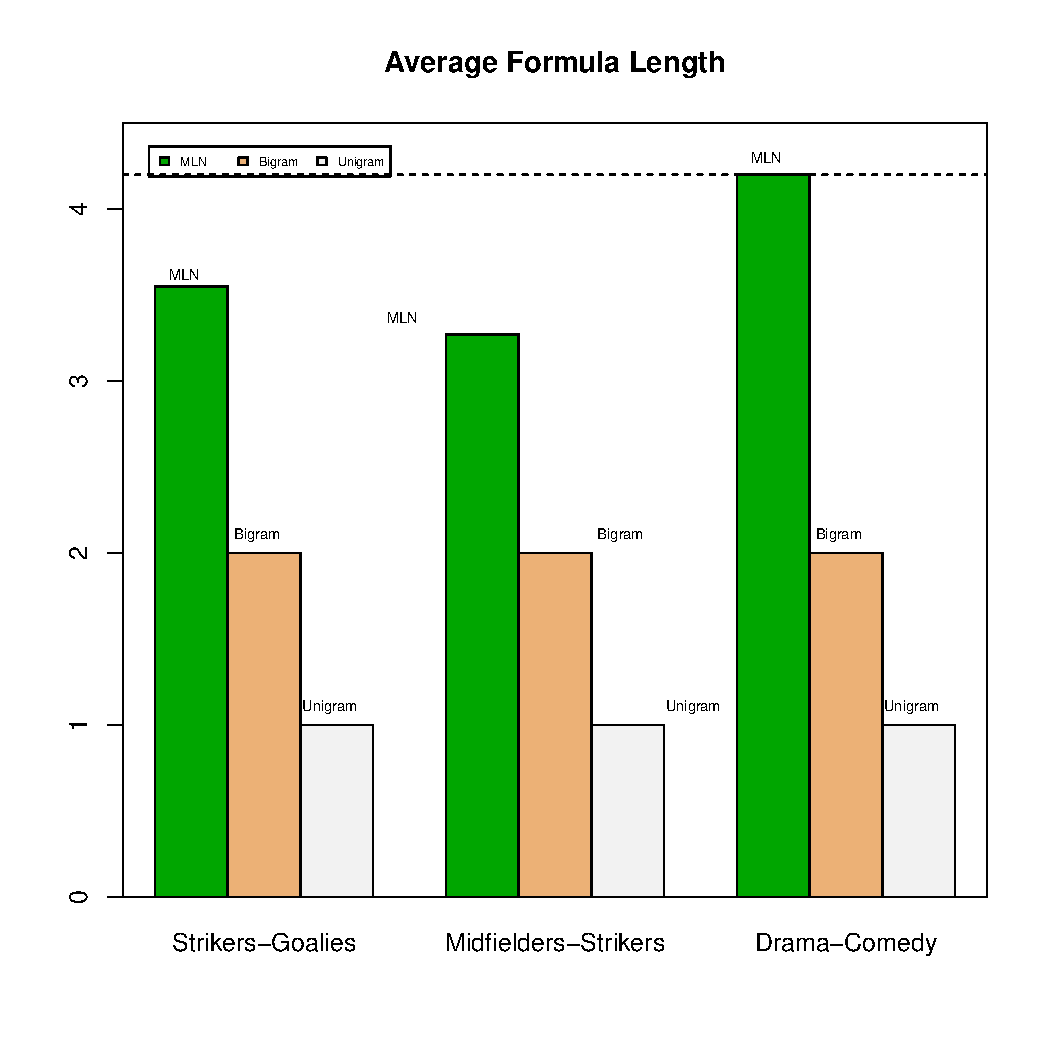
\includegraphics[width=0.48\textwidth]{Charts/formulaLength.pdf}}
							\subfigure[]{\label{fig:LowCor}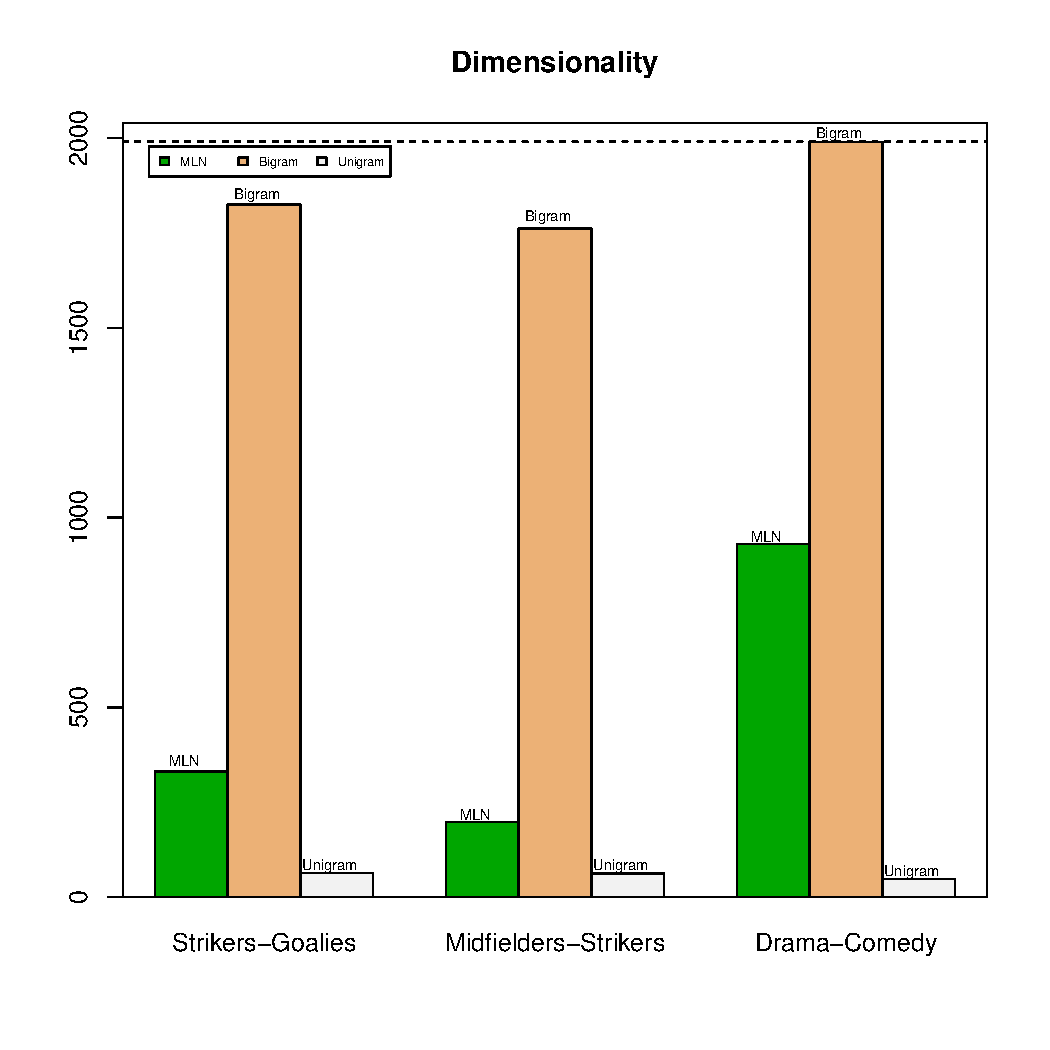
\includegraphics[width=0.5\textwidth]{Charts/dimensinality.pdf}}
							\subfigure[]{\label{fig:HighCor}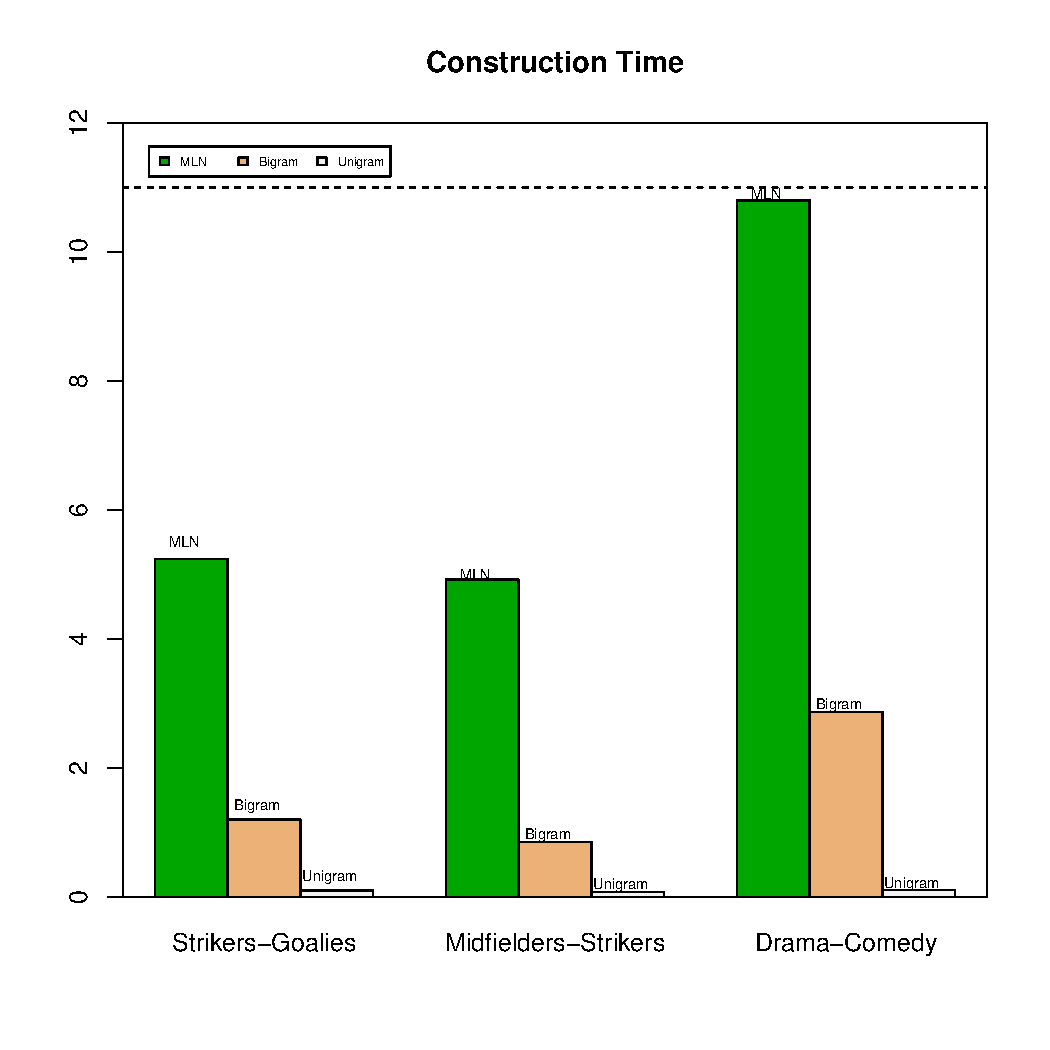
\includegraphics[width=0.5\textwidth]{Charts/ConstructionTime.pdf}}
							\caption{Comparison of complexity, dimensionality and construction time (min) for the attributes produced by different propositionalization methods}\label{fig:dimensionality}
						\end{figure}
		\subsection{Accuracy} 
		
		Figures~\ref{fig:propseSynth} and \ref{fig:propseReal} present detailed measurements of the AUC-ROC for different outlier propositionalization methods. There is no single propositionalization method that always leads to the best accuracy for all three outlier analysis methods. MLN propositionalization produces the best results on two datasets. It is always close to the maximum AUC score (never less than 0.1 AUC units away). Table~\ref{table:summary} summarizes the performance of the propositionalization methods for a fixed outlier detection algorithm. The $\mu(AUC)$ column reports the average AUC score over different datsets. A propositionalization method ``wins'' on a dataset if its AUC is at least 0.01 greater than that of others. A ``tie'' for first place earns 0.5 points. The total number of points is shown in the Wins columns. MLN-$\tf$ is revealed to be the best method in terms of average AUC, for all outlier detection methods. $\tf$ is, in a sense, the natural feature function for MLNs since the likelihood function of MLNs is defined in terms of formula grounding counts (equation 4.1). 		
		MLN-$\tf$ propositionalization scores the most wins when applied with $\lof$ or $\knn$ and a tie when applied with $\outrank$. Thus, methods that tend to treat attributes independently, such as $\lof$ and $\knn$, benefit from being provided complex attributes that summarize complex associations. Subspace analysis can utilize complex associations from bigram data, but requires much more time to do so than MLN propositionalization (see Table~\ref{table:outrank-time}).
		
		\begin{table*}
			
			\centering
			\caption{Summarizing the accuracy results of Figures~\ref{fig:propseReal} and~\ref{fig:propseSynth}: A propositionalization method is scored 1 point if it produces the best accuracy on a dataset, and 0.5 points if it ties. The table shows the total number of wins and average of AUC over all datasets.
				\label{table:summary}}
			\resizebox{0.9\textwidth}{!}{
				\begin{tabular}{|c|c|c|c|c|c|c|}
					\hline
					
					\begin{tabular}{p{4cm}}Propositionalization  $\rightarrow$\\ Outlier Detection Method $\downarrow$ \end{tabular}&\multicolumn{2}{|c|}{\begin{tabular}{p{1.5cm}}MLN-TF \end{tabular}}&\multicolumn{2}{|c|}{\begin{tabular}{p{2cm}}Bigram-IDF \end{tabular}}&\multicolumn{2}{|c|}{\begin{tabular}{p{2cm}}Unigram-TF \end{tabular}}\\\hline
					&Wins&$\mu(AUC)$&Wins&$\mu(AUC)$&Wins&$\mu(AUC)$\\\hline
					OutRank&\textbf{2.50}&\textbf{0.79}&\textbf{2.50}&0.70&1.00&0.64\\\hline
					KNN&\textbf{3.50}&\textbf{0.78}&1.50&0.67&1.50&0.67\\\hline
					LOF&\textbf{4.00}&\textbf{0.63}&1.00&0.55&1.00&0.61\\\hline
				\end{tabular}
				
			}
			
		\end{table*}
			%
			
			
									\begin{figure}
										\centering     %%% not \center
										\subfigure[ ]{\label{fig:Feature}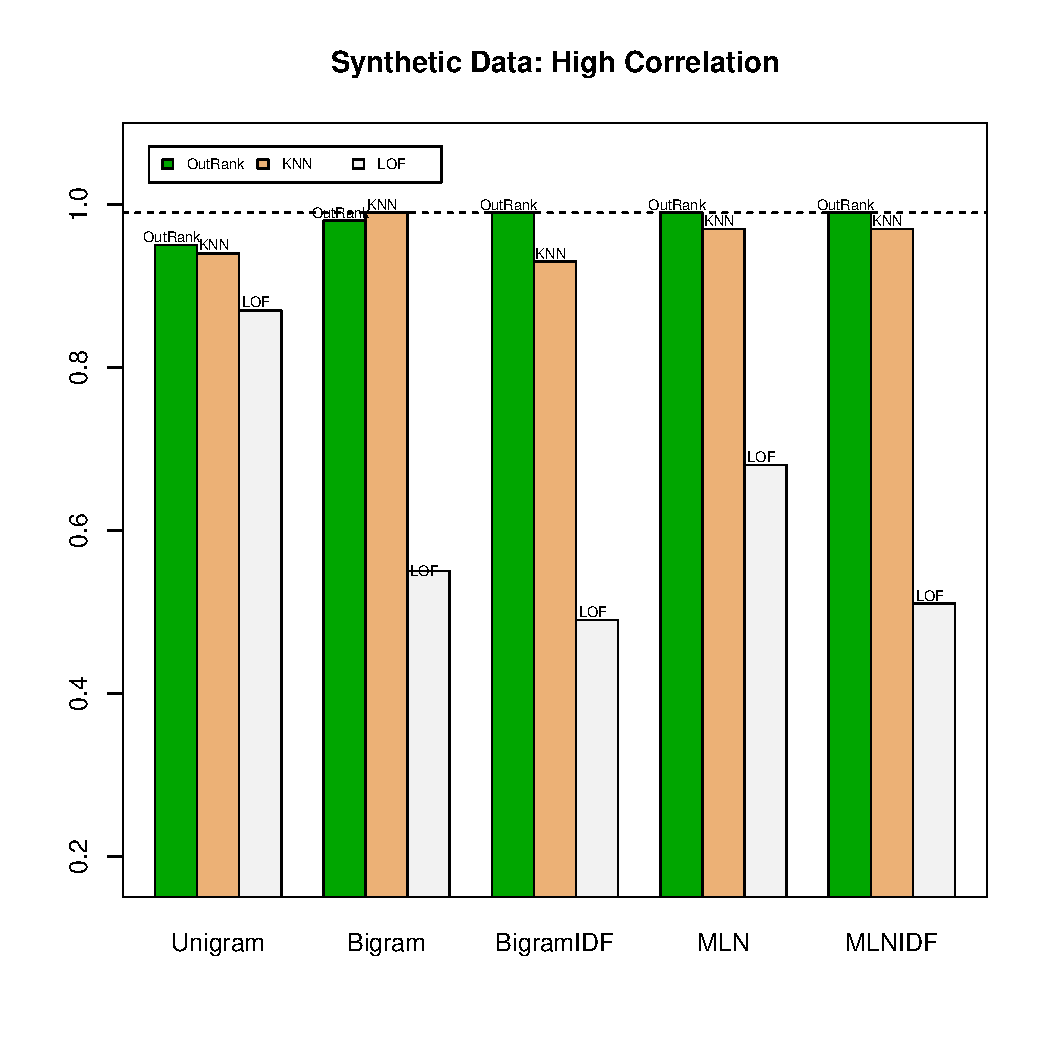
\includegraphics[width=0.48\textwidth]{Charts/highcorrelation-color.pdf}}
										\subfigure[]{\label{fig:LowCor}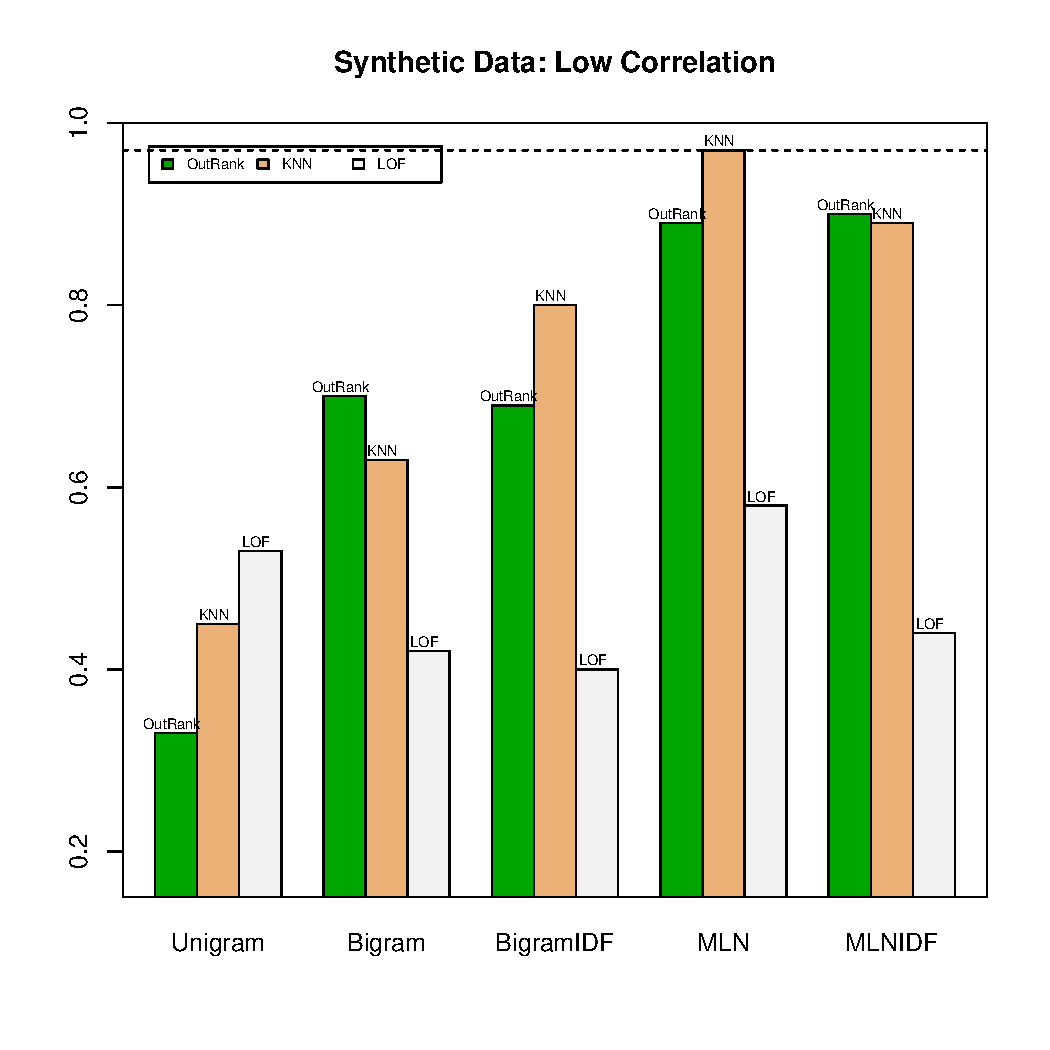
\includegraphics[width=0.5\textwidth]{Charts/lowcorrelation-color.pdf}}
										\subfigure[]{\label{fig:HighCor}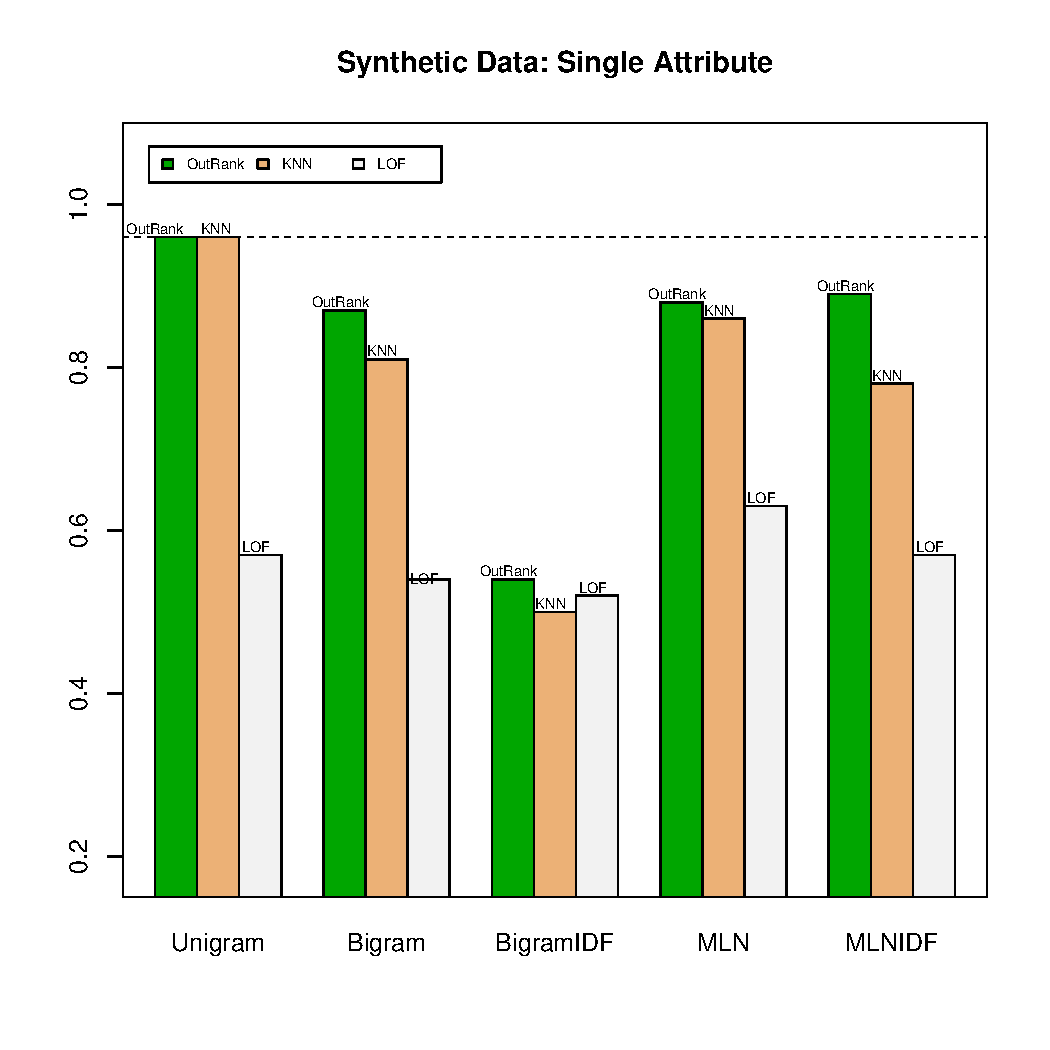
\includegraphics[width=0.5\textwidth]{Charts/SingleAttribute-color.pdf}}
										\caption{Accuracy for different Methods/Attribute Vector in the Synthetic datasets}\label{fig:propseSynth}
									\end{figure}
									
															\begin{figure}
																\centering     %%% not \center
																\subfigure[ ]{\label{fig:Feature}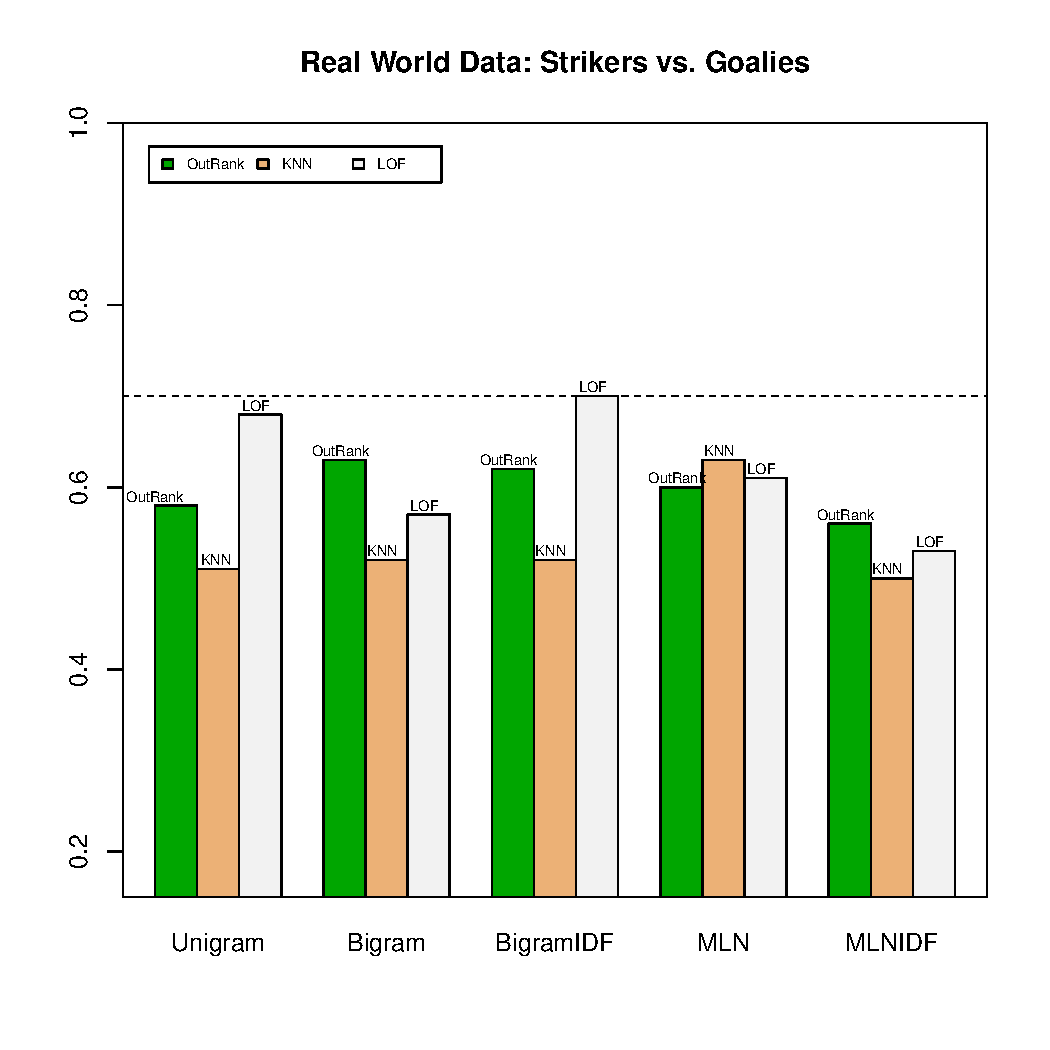
\includegraphics[width=0.48\textwidth]{Charts/strikersx.pdf}}
																\subfigure[]{\label{fig:LowCor}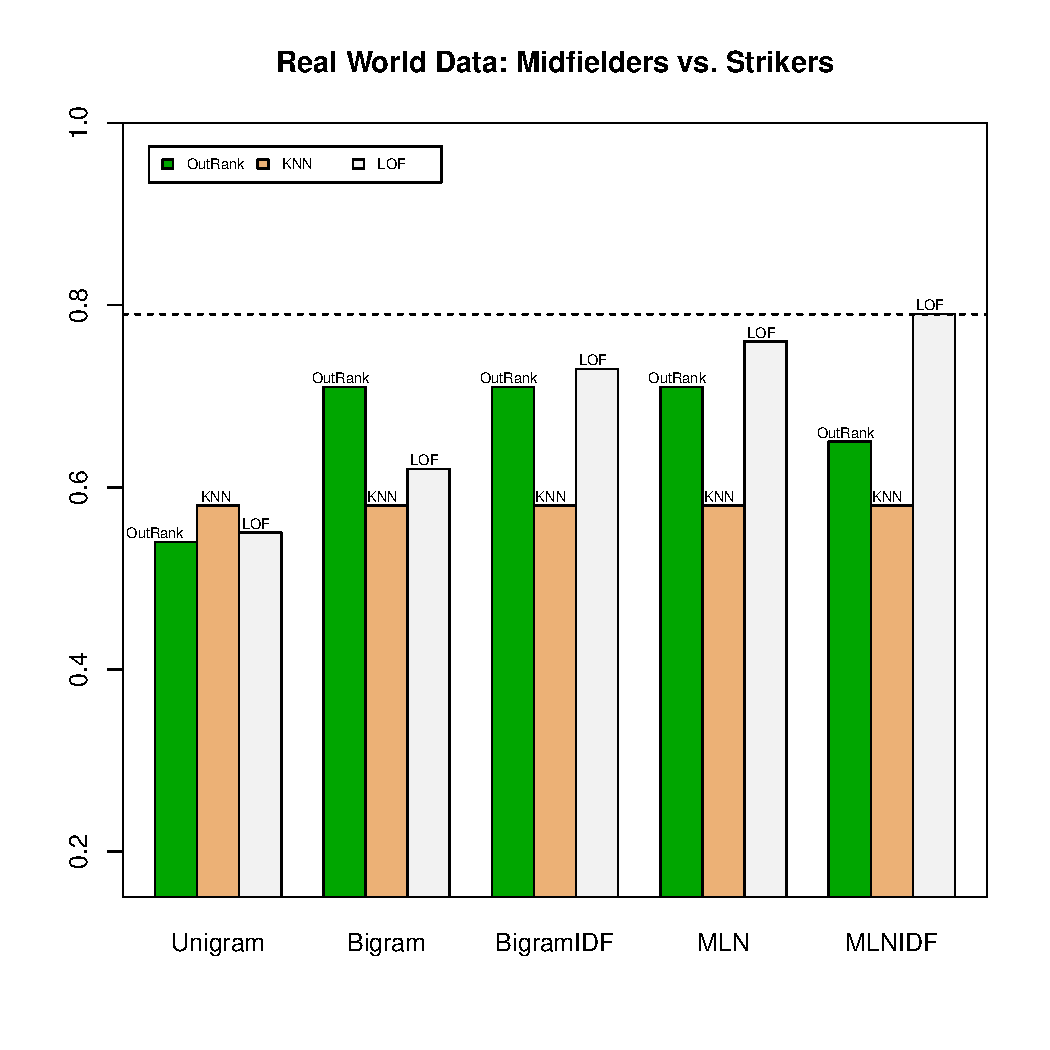
\includegraphics[width=0.5\textwidth]{Charts/midfielder-color.pdf}}
																\subfigure[]{\label{fig:HighCor}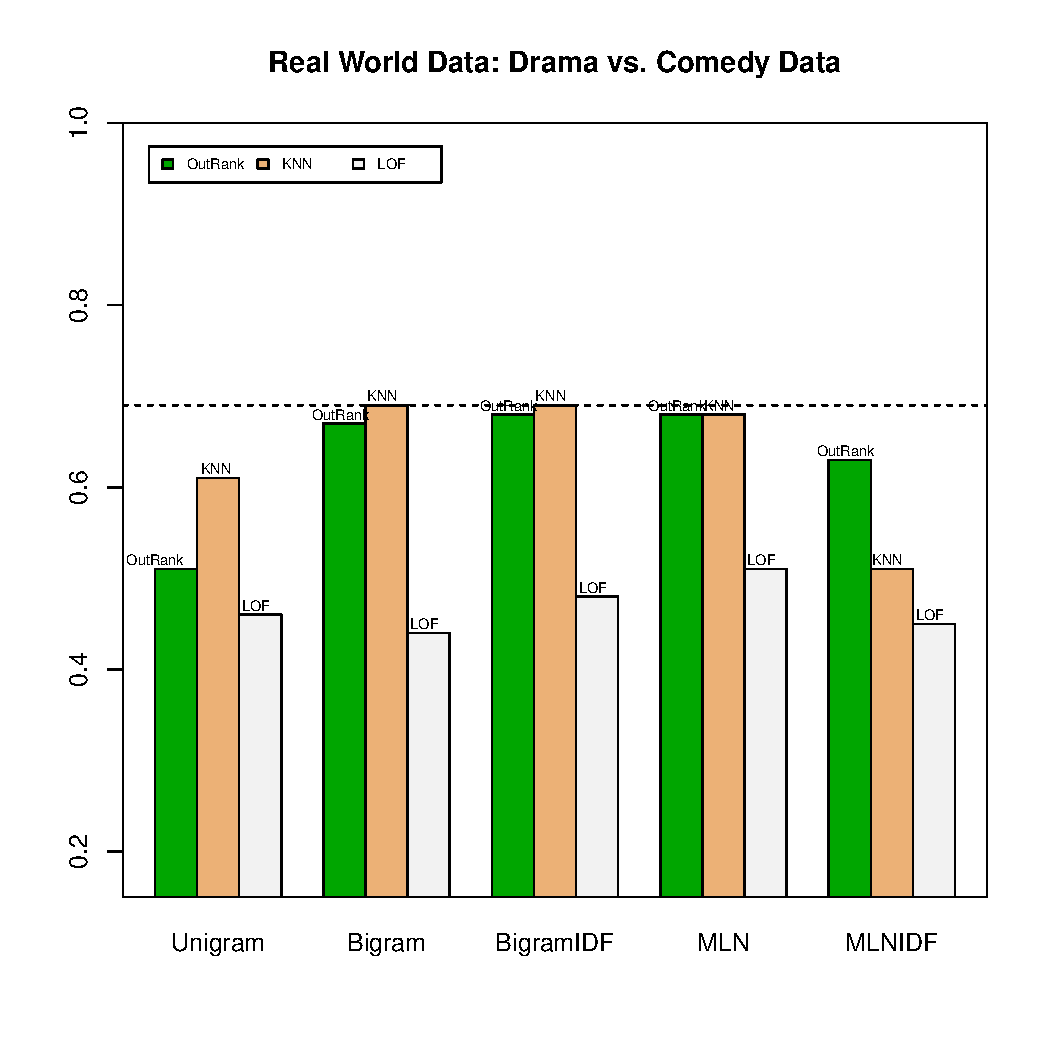
\includegraphics[width=0.5\textwidth]{Charts/imdb-color.pdf}}
																\caption{Accuracy for different Methods/Attribute Vector in the Real World datasets}\label{fig:propseReal}
															\end{figure}
									
								
			
			
			
			
%			
%											\begin{figure}
%												\centering
%												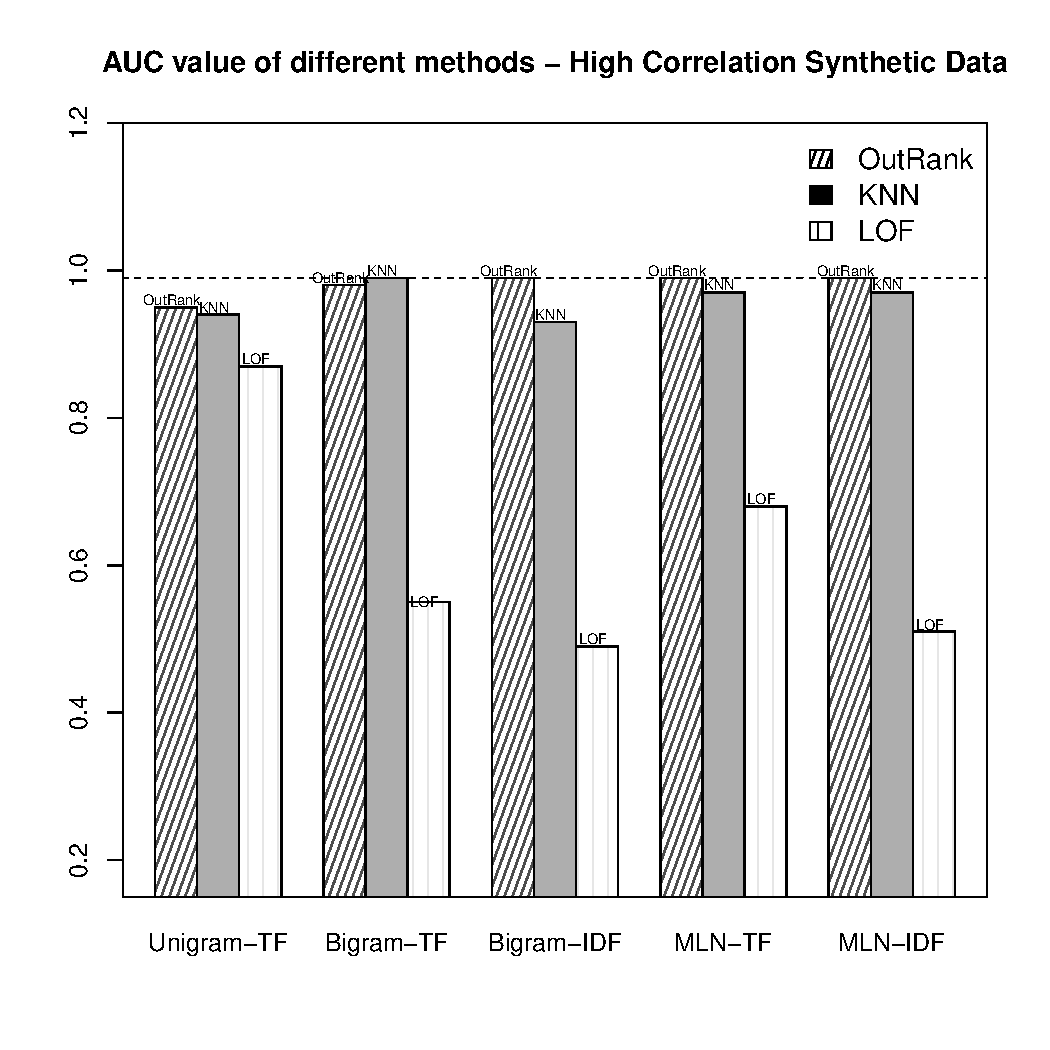
\includegraphics[width=0.6\textwidth] {Charts/highcorrelation.pdf}
%												\caption{System Flow
%													\label{main:b}}
%											\end{figure}
%											
%				
%						\end{figure}
%								\begin{figure}
%									\centering
%									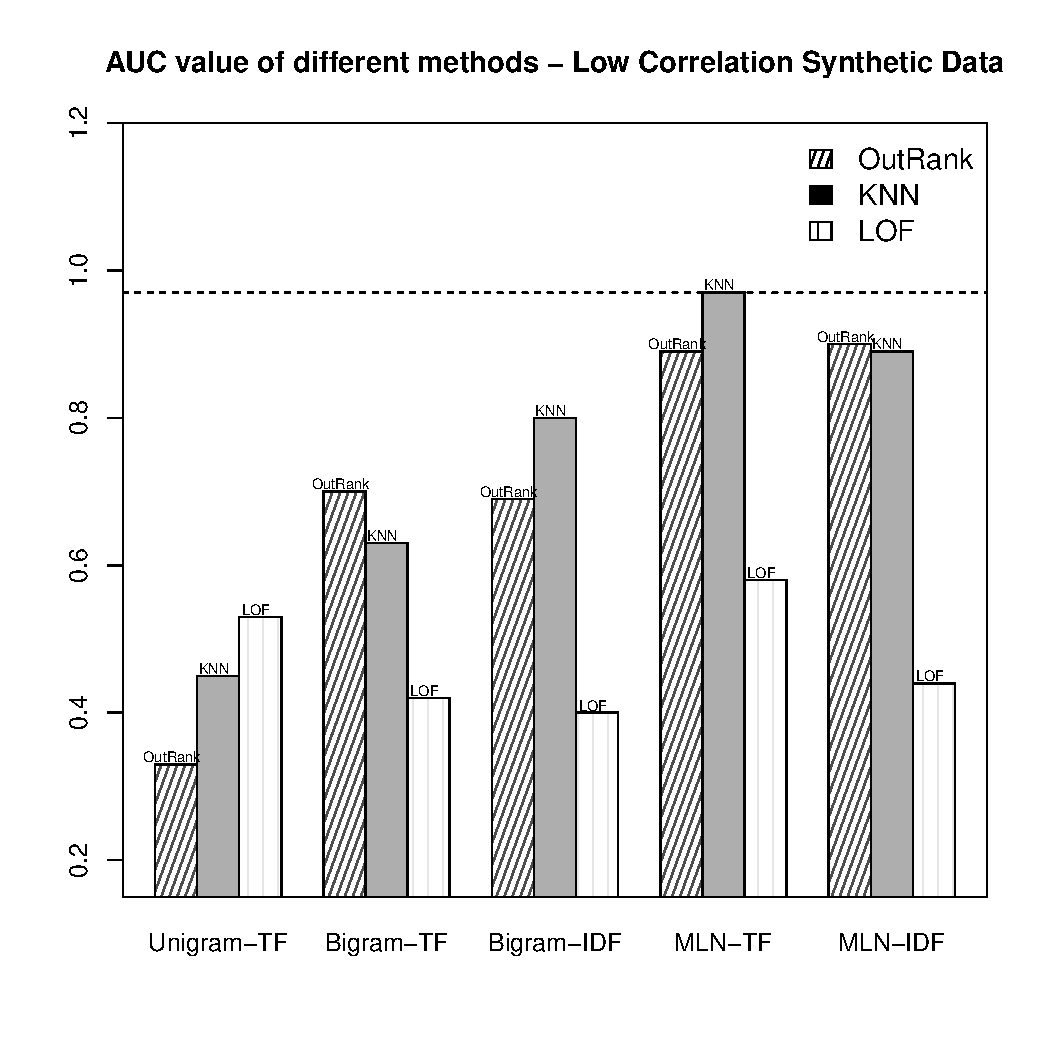
\includegraphics[width=0.6\textwidth] {Charts/lowcorrelation.pdf}
%									\caption{System Flow
%										\label{main:b}}
%								\end{figure}
%												
%												
%												
%					\begin{figure}
%						\centering
%						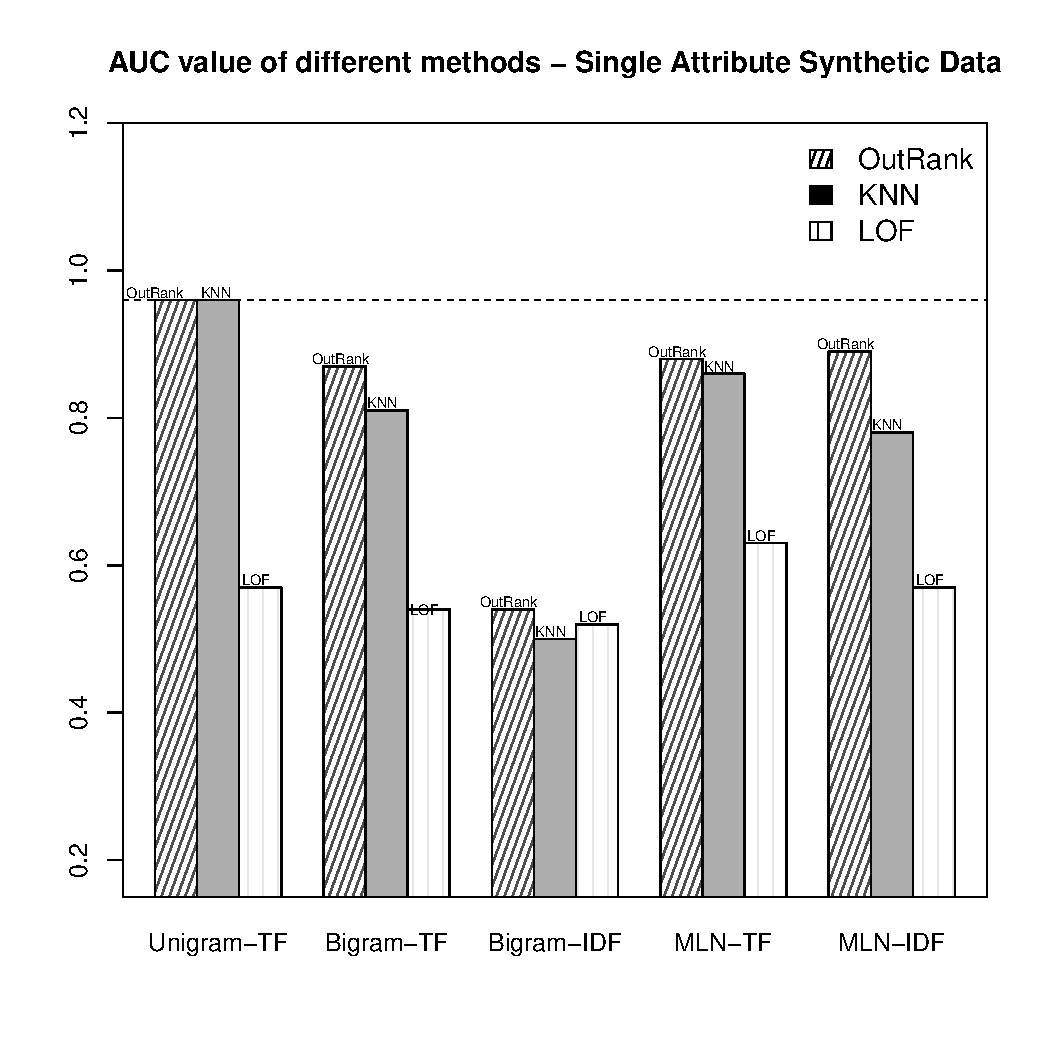
\includegraphics[width=0.6\textwidth] {Charts/SingleAttribute.pdf}
%						\caption{System Flow
%							\label{main:b}}
%					\end{figure}
					
					
			
			

			\section{Comparison With Propositionalization for Supervised Outlier Detection and Log-Likelihood} 
	
			In this section we compare our novel MLN propositionalization method
			with a previous propositionalization method that was developed for supervised classification problems. Since, to our knowledge, all previous propositionalization methods are for classification problems, in this section only we consider {\em supervised} outlier detection, where examples are labelled as ``normal'' and ``abnormal''. Given the ground truth labels, supervised outlier detection can be treated as a special case of classification \cite{Hodge2004}. Supervised outlier detection serves as a benchmark of the accuracy of unsupervised outlier detection: if the unsupervised method comes close to the accuracy of the supervised method, this indicates a good performance of the unsupervised method. 
			
			We report experiments with the state-of-the-art Treeliker propositionalization method \cite{kuzelka2008}. We used the implementation of Treeliker available in the ClowdFlows platform \cite{Kranjc2012}, which supports the MySQL data format. The HiFi algorithm from \cite{kuzelka2008} has been used with minimum frequency specified as 0.2, maximum size of features to be 10 and sample size as 5. We train and test Treeliker on the same dataset with ground truth labels as classification target. So the way we use Treeliker gives it two advantages over MLN propositionalization: It sees the ground truth labels, and it is tested on the training data. On almost all real-world datasets, this translates into a higher AUC score, except for the Striker-Midfielder problem using $\lof$ (0.61 for MLN vs. 0.56 for Treeliker). MLN propositionalization comes close to the Treeliker score, the only substantial difference occurs with $\lof$ on the Striker-Goalie problem (0.76 for MLN vs. 0.84 for Treeliker).  On the synthetic data, the MLN method performs even better, beating the Treeliker propositionalization by a substantial margin. Given the advantages for the supervised setting, this is a very good performance for MLN propositionalization. We emphasize that this is not a criticism of Treeliker as a propositionalization method, because it is not designed for outlier detection problems. Rather, our conclusion is that new methods provide value for the problem of propositionalization for outlier detection. 
			
			\begin{table*}
				
				\centering
				\resizebox{0.6\textwidth}{!}{
					\begin{tabular}{llcccc}
						\hline
						
						Database&\begin{tabular} {p{1.5cm}}Outlier Method\end{tabular}&\begin{tabular} {p{1.5cm}} Treeliker \\ AUC value \end{tabular}& \begin{tabular} {p{1.5cm}} MLN-TF \\ AUC value \end{tabular}&\begin{tabular}{p{1.5 cm}}%\\\hline
						%	Treeliker\\VectorSize
					%	\end{tabular}&\begin{tabular}{p{1.5 cm}}
					%	MLN-TF\\VectorSize
					\end{tabular}\\\hline
				%	Single Attribute&OutRank& NA&\textbf{0.88}&303&6\\\hline
					Single Attribute&KNN& 0.65&\textbf{0.86}\\\hline%&303&6\\\hline
					Single Attribute&LOF& 0.53&\textbf{0.63}\\\hline%&303&6	
				%	High Correlation&OutRank& NA&\textbf{0.99}&302&6\\\hline
					High Correlation&KNN& 0.66&\textbf{0.97}\\\hline%&302&6\\\hline
					High Correlation&LOF& 0.57&\textbf{0.68}\\\hline%&302&6	\\\hline
			%		Low Correlation&OutRank& NA&\textbf{0.89}&302&6\\\hline
					Low Correlation&KNN& 0.65&\textbf{0.97}\\\hline%&302&6\\\hline
					Low Correlation&LOF& 0.56&\textbf{0.58}\\\hline%&302&6	\\\hline
					
			%		Striker Goalie&OutRank& NA&\textbf{0.71}&3,620&331\\\hline
					Striker Goalie &KNN& \textbf{0.6}&0.58\\\hline%&3,620&331\\\hline
					Striker Goalie &LOF& \textbf{0.84}&0.76\\\hline%&3,620&331	\\\hline
			%		Midfielder Striker&OutRank& NA&\textbf{0.6}&5,093&198\\\hline
					Midfielder Striker&KNN& \textbf{0.65}&0.63\\\hline%&5,093&198\\\hline
					Midfielder Striker&LOF&0.56&\textbf{0.61}\\\hline%&5,093&198	\\\hline
					
				\end{tabular}
				
			}
			\caption{Accuracy of Treeliker for different databases and outlier techniques. Bold values represent the cases where Treeliker outperforms other methods. 
				\label{table:Treeliker}}
		\end{table*}
%		\subsection{Result of Log-likelihood}
%		The log-likelihood method \cite{FatemehRiahi2013a} combines learned MLN weights with MLN structure. The outlier score is the weighted sum of formula groundings for each potential outlier individual. The accuracy of the log-likelihood method is similar to that of Markov Logic propositionalization, depending on the outlier analysis method (e.g., for $\outrank$ and $\knn$ the average AUC difference is 0.01 in favor of log-likelihood, for $\lof$ log-likelihood does much better; the average of AUC difference is 0.17).
%		Table~\ref{table:Metric Comparison} shows the performance of Log-likelihood in different datasets.
%		\begin{table}[!htbp]
%			
%			
%			\centering
%			\resizebox{0.5\textwidth}{!}{
%				\begin{tabular}{|l|l|}
%					\hline
%					Dataset & \loglikelihood\\ \hline
%					
%					Synthetic Data-High Correlation &0.98 \\ \hline
%					Synthetic Data-Low Correlation &0.95 \\ \hline
%					Synthetic Data-Single Feature&0.98 \\ \hline
%					Real Data-Strikers vs. Goalies& 0.65\\ \hline
%					Real Data-Midfielders vs. Strikers&0.64 \\ \hline
%					Real Data-Drama vs. Comedy&0.63 \\ \hline
%				\end{tabular}}
%				\caption{$\auc$ of Log-likelihood in different datasets. 
%					%For relationships please see text.
%					\label{table:Metric Comparison}}
%			\end{table}
	\section{Conclusion}		
	In this chapter we developed a pipeline propositionalization approach where the information from multiple data tables is summarized in a single data table. The key step is to find a set of relevant logical formulas that define conjunctive attributes of potential outlier individuals as sum. We utilized Markov Logic Network learning for this task. In an empirical comparison with the baseline wordification approach of enumerating all conjunctive formulas up to length 2, Markov Logic propositionalization showed several advantages: 1) The set of formulas learned was substantially smaller, leading to smaller data tables and faster outlier detection. 2) The formulas learned were longer, representing more complex relational patterns. 3) For a fixed single-table outlier analysis method, the average detection accuracy was higher.
	
	We view this work as an initial step in the topic of propositionalization for outlier detection, there are several fruitful directions for future work. While Markov Logic networks are a prominent generative model class for relational data, our approach can be used with  other generative models; this opens a new application area for statistical-relational learning. Dimensionality reduction techniques can be employed after propositionalization to reduce the size of the data tables before outlier detection methods are used. Propositionalization algorithms that were developed for classification could be adapted for unsupervised outlier detection by using a feature selection score that is relevant for outlier detection, rather than supervised classification.
	
	Another direction for future work is to leverage graph-based descriptive features in our generative model learning process.
	These features proved to be efficient in discovering patterns for anomaly detection task in ODDBALL~\cite{Akoglu2010}. Examples of such features in our datasets include: number of matches a player has played, number of reviews a movie has received, and features related to the extent of interaction between players.
